\documentclass[tikz,border=7pt]{standalone}
\usepackage{amsmath,amssymb}
\usepackage[scaled]{helvet}
\renewcommand{\familydefault}{\sfdefault}
\usetikzlibrary{arrows.meta,backgrounds,calc,fit,positioning,shapes.geometric}
\definecolor{bpink}{HTML}{172033}
\definecolor{bpblue}{HTML}{2A78D6}
\definecolor{bporange}{HTML}{E56A32}
\definecolor{bpgreen}{HTML}{168A65}
\definecolor{bppurple}{HTML}{7A5CC7}
\definecolor{bpred}{HTML}{C94A4A}
\definecolor{bpmuted}{HTML}{667085}
\definecolor{bpgrid}{HTML}{D8DEE8}
\definecolor{bpsurface}{HTML}{F8FAFC}
\tikzset{
  var/.style={circle,draw=bpblue,fill=bpblue!10,line width=.9pt,minimum size=8mm,font=\small\bfseries,text=bpink},
  factor/.style={rectangle,rounded corners=1.5pt,draw=bporange,fill=bporange!14,line width=.9pt,minimum size=6.8mm,font=\small\bfseries,text=bpink},
  constraint/.style={rectangle,rounded corners=1.5pt,draw=bpred,fill=bpred!12,line width=.9pt,minimum size=6.8mm,font=\small\bfseries,text=bpink},
  edge/.style={draw=bpmuted!75,line width=.9pt},
  msgvf/.style={-{Latex[length=2.2mm]},draw=bpblue,line width=1.35pt},
  msgfv/.style={-{Latex[length=2.2mm]},draw=bporange,line width=1.35pt},
  label/.style={font=\scriptsize,text=bpmuted,align=center},
  title/.style={font=\bfseries\large,text=bpink},
  card/.style={draw=bpgrid,fill=bpsurface,rounded corners=7pt,line width=.7pt},
}

\begin{document}
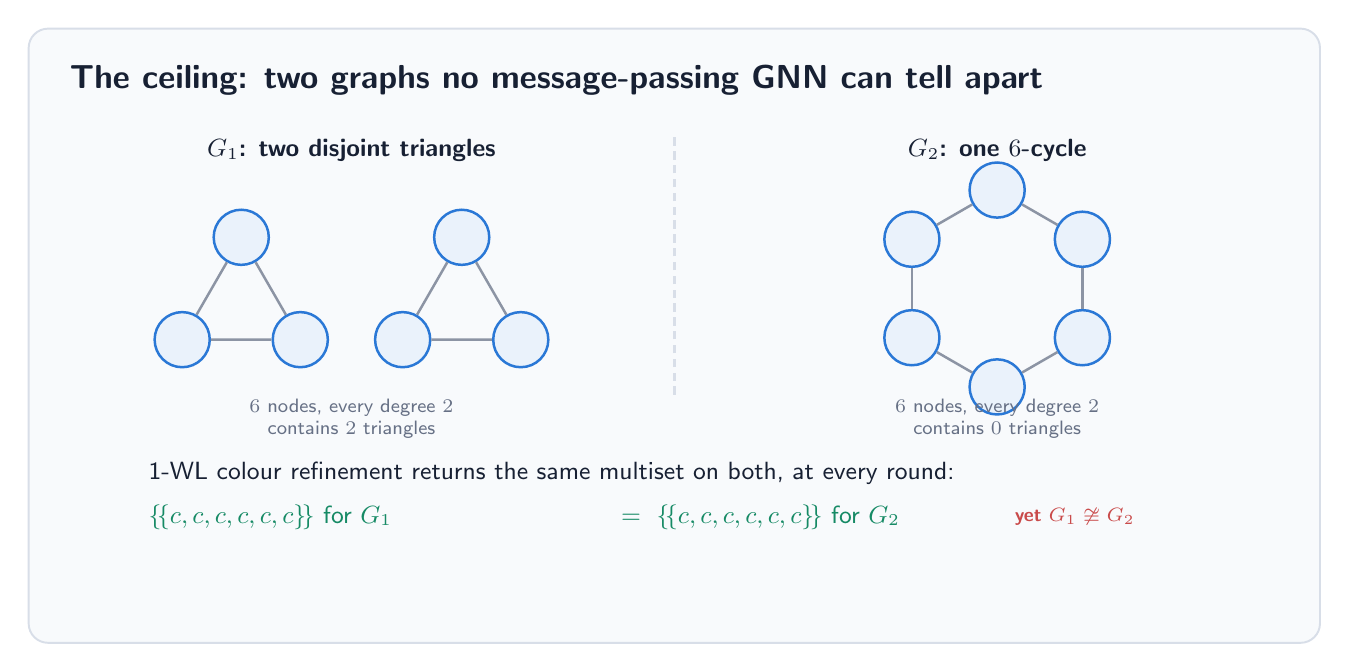
\begin{tikzpicture}[font=\sffamily]
  \node[card,minimum width=16.4cm,minimum height=7.8cm] at (7.4,2.6) {};
  \node[title,anchor=west] at (-.4,5.85) {The ceiling: two graphs no message-passing GNN can tell apart};

  % ---- left: two triangles ----
  \node[text=bpink,font=\small\bfseries] at (3.3,4.95) {$G_1$: two disjoint triangles};
  \foreach \k/\cx in {1/1.9, 2/4.7}{
    \node[var,minimum size=7mm] (a\k) at (\cx,3.85) {};
    \node[var,minimum size=7mm] (b\k) at (\cx-.75,2.55) {};
    \node[var,minimum size=7mm] (c\k) at (\cx+.75,2.55) {};
    \draw[edge] (a\k)--(b\k)--(c\k)--(a\k);
  }
  \node[label,align=center] at (3.3,1.55) {$6$ nodes, every degree $2$\\contains $2$ triangles};

  % ---- right: 6-cycle ----
  \node[text=bpink,font=\small\bfseries] at (11.5,4.95) {$G_2$: one $6$-cycle};
  \foreach \i in {0,...,5}{
    \pgfmathsetmacro{\ang}{90+60*\i}
    \node[var,minimum size=7mm] (h\i) at ({11.5+1.25*cos(\ang)},{3.2+1.25*sin(\ang)}) {};
  }
  \foreach \i/\j in {0/1,1/2,2/3,3/4,4/5,5/0}{ \draw[edge] (h\i)--(h\j); }
  \node[label,align=center] at (11.5,1.55) {$6$ nodes, every degree $2$\\contains $0$ triangles};

  \draw[bpgrid,line width=.9pt,densely dashed] (7.4,1.85) -- (7.4,5.15);

  \node[anchor=west,text=bpink,font=\small] at (.6,.85)
    {1-WL colour refinement returns the same multiset on both, at every round:};
  \node[anchor=west,font=\small,text=bpgreen] at (.6,.30)
    {$\{\!\{c,c,c,c,c,c\}\!\}$ for $G_1$};
  \node[anchor=west,font=\small,text=bpgreen] at (6.6,.30)
    {$=\ \{\!\{c,c,c,c,c,c\}\!\}$ for $G_2$};
  \node[anchor=west,text=bpred,font=\scriptsize\bfseries] at (11.6,.30)
    {yet $G_1\not\cong G_2$};
\end{tikzpicture}
\end{document}
